\documentclass[12pt,a4paper]{article}
\usepackage[utf8]{inputenc}
\usepackage[ngerman]{babel}
\usepackage[left=2.5cm,right=2.5cm,top=3cm,bottom=2cm]{geometry}
\author{Pauline Speckmann}
\usepackage{graphicx}
\usepackage{booktabs}
\usepackage{adjustbox}

\usepackage{fancyhdr}
\pagestyle{fancy}
\fancyhf{}
\fancyhead[l]{Digitalisierung Vorlesung 7 $-$ Zusammenfassung von Pauline Speckmann}
\fancyhead[r]{\thepage}


\begin{document}

\setcounter{section}{6}
\section{Geschäftsmodellinnovation und digitale Plattformen}


\vspace*{1cm}
\subsection{Digitale Technologien und Geschäftsmodellinnovation} %%%%%%%%%%%%%%%%%%%%%%%%%%%%%%%%%%%%%%%%%%%%%%%%%%%%%%%%%%%%%%%%%%%%%
\begin{itemize}
   \item \textbf{Geschäftsmodellinnovation:}\\
         Verändern sich mindestens zwei Dimensionen eines Geschäftsmodells signifikant, spricht man von einer Geschäftsmodellinnovation.

   \item \textbf{Vergleich traditioneller und neuartiger, digitaler Wirtschaft:}
   \item[] 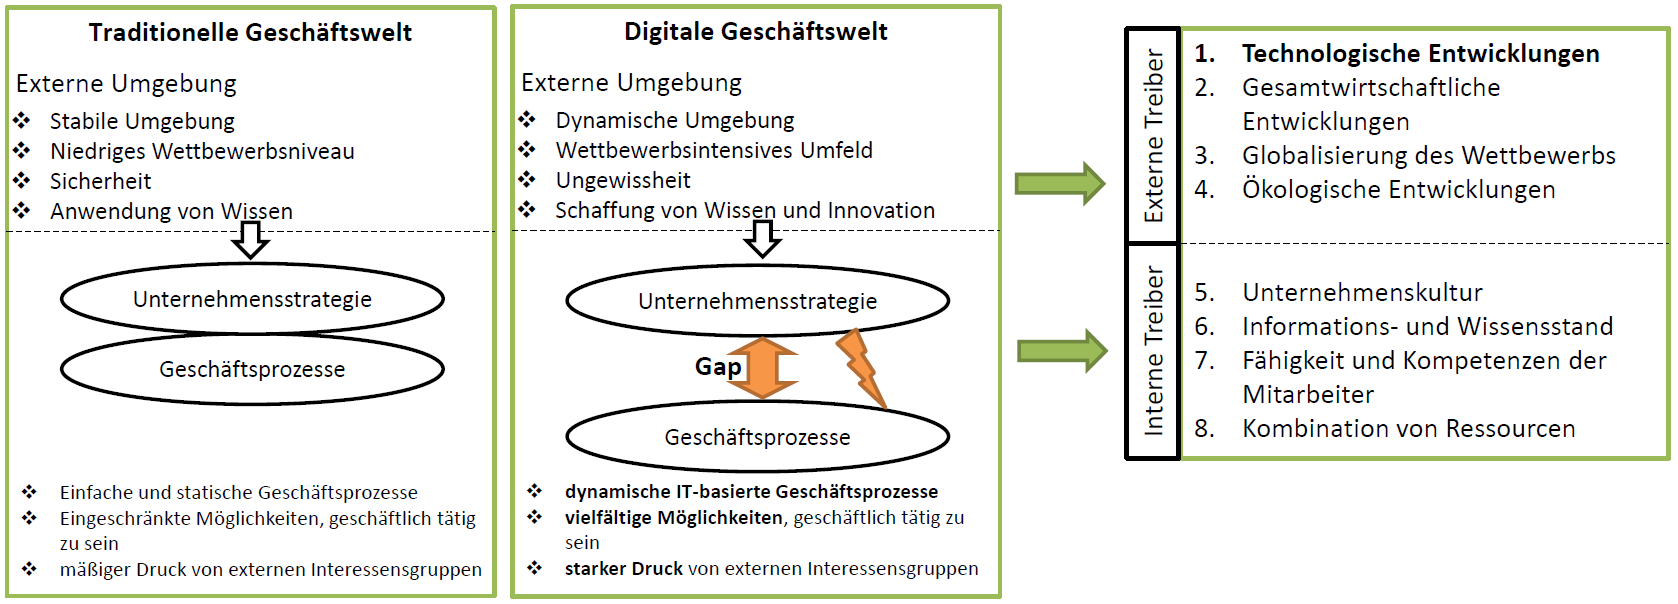
\includegraphics[scale=0.35]{TraditionellVsDigital.png}
   
   \item \textbf{Innovationsgrade der Geschäftsinnovation:} \vspace*{-0.5cm}
   \item[] \begin{minipage}[t]{0.35\textwidth} \vspace*{0cm}
               \begin{itemize}
		            \item \textbf{Radikale Innovation:}\\
		                  Fundamentale Veränderungen in angrenzenden oder neuen Märkten (Hohes Chancen–Risiko Verhältnis)
		            \item \textbf{Inkrementelle Innovation:}\\
		                  Geringfügige Veränderungen, die etablierte Produkt-Markt-Felder fortführen (Geringes Chancen–Risiko Verhältnis)
		         \end{itemize}
            \end{minipage} \begin{minipage}[t]{0.05\textwidth} \vspace*{0cm}
               $\ $ \\
            \end{minipage} \begin{minipage}[t]{0.5\textwidth} \vspace*{0cm}
               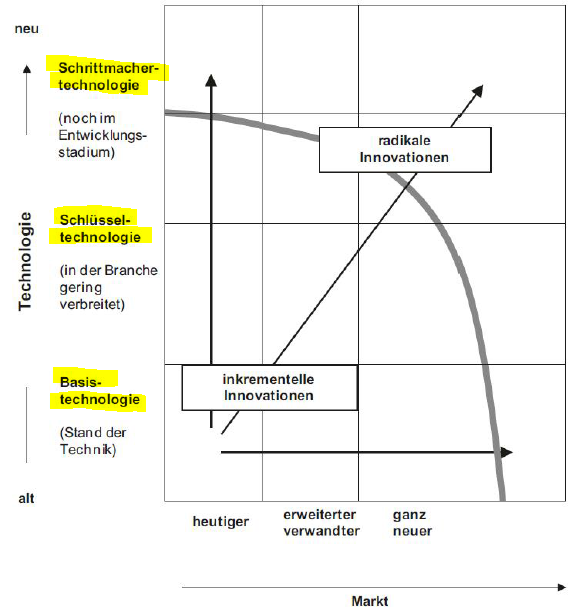
\includegraphics[scale=0.55]{InnovationsgradeH.png}
            \end{minipage}
   
   \newpage
   \item \textbf{Potenziale digitaler Technologien für Geschäftsmodellinnovation:}
         \begin{itemize}
            \item ($\uparrow$) Weniger gebundene Innovationen
            \item ($\rightarrow$) Weniger Grenzen zwischen Innovationsprozess und -ergebnissen
            \item ($\leftarrow$) Mehr Innovationsakteure
         \end{itemize}

   \item \textbf{Werttreiber digitaler Geschäftsmodelle:}
         \begin{itemize}
            \item \textbf{Novelty} (Neuigkeitsgehalt):\\
                  Wie soll das bestehendes Geschäftsmodell verändert werden und sich somit von der Konkurrenz abgrenzen?
            \item \textbf{Lock-In} (Kunden-/ Lieferantenbindung):\\
                  Wie können wir Kunden und Partner an das Geschäftsmodell binden?
            \item \textbf{Complementarities} (Komplementaritäten):\\
                  Wo lassen sich Synergien mit bestehenden Kompetenzen schaffen?
            \item \textbf{Efficiencies} (Effizienz):\\
                  In wie fern ist die neue Architektur günstiger und/oder liefert einen höheren Wert für den Kunden?
         \end{itemize}
   
   \item \textbf{Drei zentrale Komponenten eines digitalen Geschäftsmodells:}
   \item[] 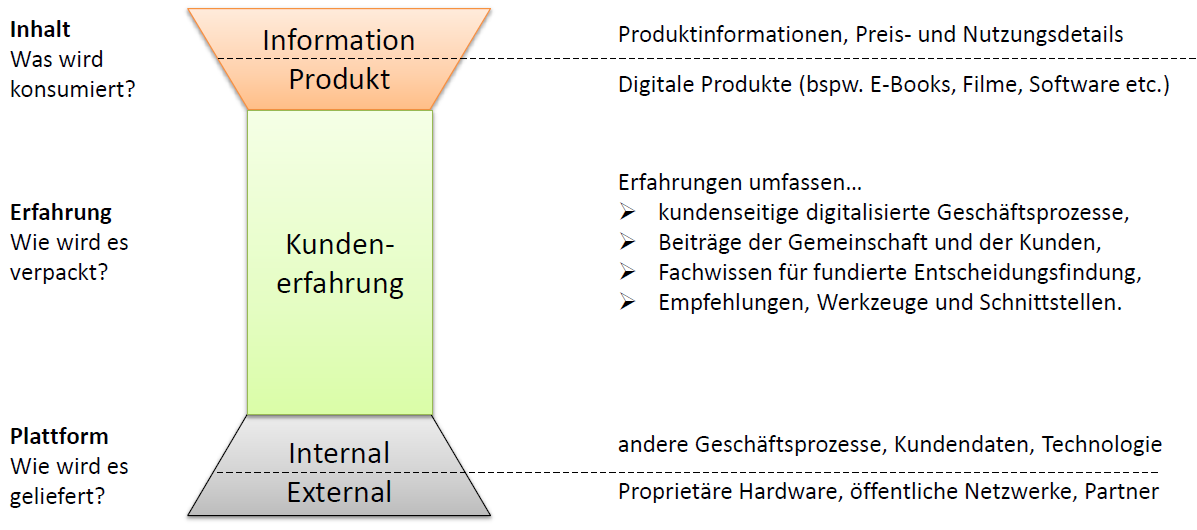
\includegraphics[scale=0.47]{DreiKomponenten.png}
\end{itemize}


\vspace{1cm}
\subsection{Digitale Plattformen} %%%%%%%%%%%%%%%%%%%%%%%%%%%%%%%%%%%%%%%%%%%%%%%%%%%%%%%%%%%%%%%%%%%%%%%%%%%%%%%%%%%%%%%%%%%%%%%%%%%%
\begin{itemize}
   \item \textbf{Prinzip:}\\
         Eine Plattform basiert darauf wertschöpfende Interaktionen zwischen externen Produzenten und Konsumenten zu ermöglichen.
   
   
   \newpage
   \item \textbf{Vier Kernelemente digitaler Plattformen:}
   \item[] 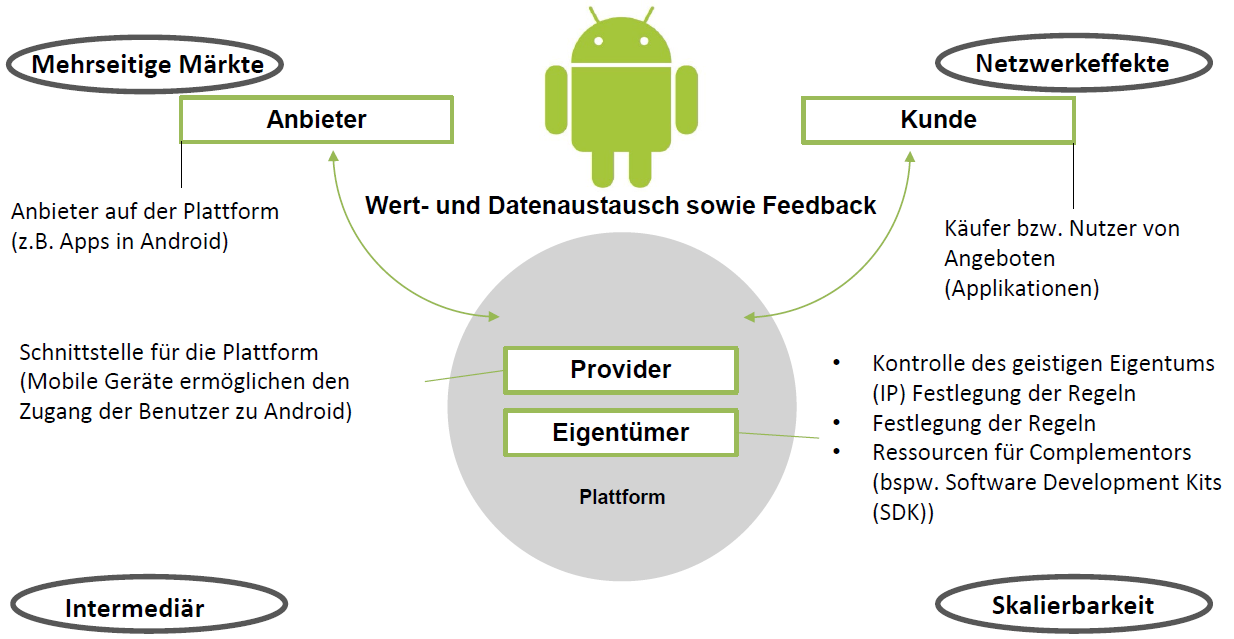
\includegraphics[scale=0.42]{VierKernelemente.png}
   
   \item \textbf{Eigenschaften einer digitalen Plattform:}
         \begin{itemize}
            \item Ist ein Nexus aus Regeln und Architektur
            \item Ist offen, erlaubt geregelte Teilnahme
            \item Fördert aktiv (positive) Interaktionen zwischen verschiedenen Partnern in einem mehrseitigen Markt
            \item Skaliert viel schneller als ein Pipeline-Geschäft, weil es nicht zwingend die Kosten der externen Produktion trägt
         \end{itemize}
   
   \item \textbf{Netzwerkeffekte digitaler Plattformen:}
         \begin{itemize}
            \item \textbf{Direkte Netzwerkeffekte:}\\
                  Mehr Nutzer eines Produkts oder Services führen zu größerem Nutzen für alle Mitglieder des Netzwerkes.
            \item \textbf{Indirekte Netzwerkeffekte:}\\
                  Mehr Nutzer eines Produkts oder Services erhöhen den Wert von Komplementärprodukten auf der Plattform.Mehr Komplementärprodukte machen die Plattform attraktiver für Nutzer.
         \end{itemize}
   
   \item \textbf{Architektur digitaler Plattformen $–$ Sozio-technische Perspektive:}
   \item[] 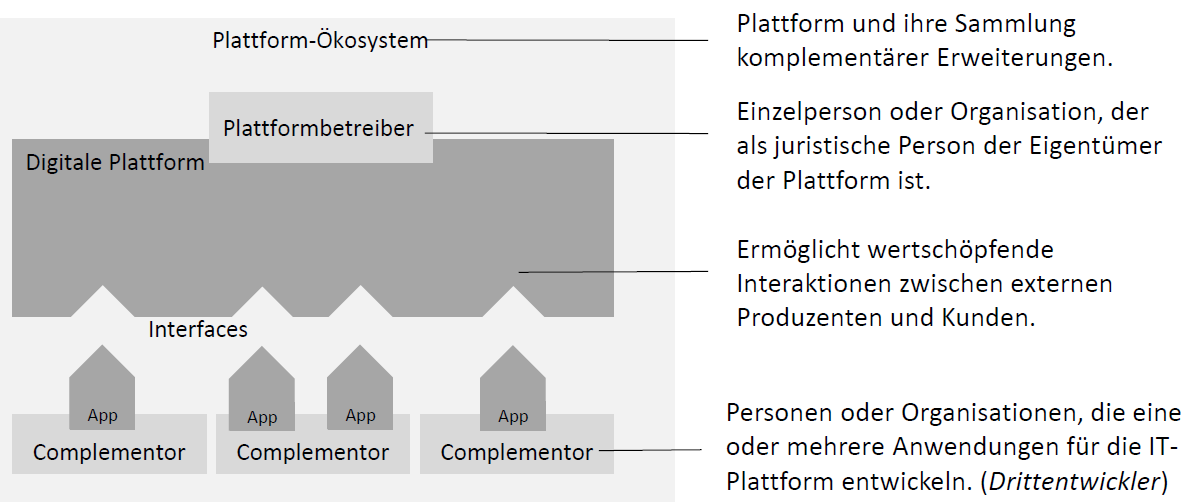
\includegraphics[scale=0.43]{ArchitekturDigitalerPlattformen.png}
   \item[] Die Bereitstellung von API \textit{Application Programming Interfaces} (im Bereich der \textit{Interfaces}) durch den Plattformbesitzer zur Anbindung von Applikationen in die Plattform ermöglicht:
         \begin{itemize}
            \item Möglichkeit der Zusammenarbeit mit externen Akteuren
            \item Reduzierung von Integrationskomplexität
            \item Möglichkeit der offenen Innovation
            \item Erhöhung der Reichweite und Präsenz am Markt
         \end{itemize}
   
   \item \textbf{Charakteristika digitaler Plattformen:}
         \begin{itemize}
            \item \textbf{Henne-Ei Problematik:}\\
                  Das Henne-Ei-Problem beschreibt die Herausforderung, Nutzer einer Marktseite für die Plattform zu gewinnen, bevor eine kritische Masse an anderen Nutzern einer anderen Marktseite präsent ist.
            \item \textbf{Multi Homing:}\\
                  Multihoming beschreibt den parallelen Einsatz mehrerer Plattformen auf einer der Nutzerseiten.
                  Plattformbetreiber wollen Multihoming vermeiden, um Wettbewerbsvorteile zu erzielen (z.B. durch exklusive Inhalte).
            \item \textbf{Winner-takes-it-all:}\\
                  Winner-takes-it-all-Effekte entstehen dadurch, dass sich durch die selbst\-ver\-stärk\-en\-den Wachstumseffekte meist ein dominierender Anbieter durchsetzt, der die konkurrierenden Betreiber in eine Nische oder ganz vom Markt verdrängt.
         \end{itemize}
\end{itemize}


\newpage
\subsection{QUIZFRAGEN} %%%%%%%%%%%%%%%%%%%%%%%%%%%%%%%%%%%%%%%%%%%%%%%%%%%%%%%%%%%%%%%%%%%%%%%%%%%%%%%%%%%%%%%%%%%%%%%%%%%%%%%%%%%%%%
\begin{itemize}
   \item Für die Plattform \emph{Ebay} bestehen Indirekte Netzwerkeffekte zwischen Käufer und Händler.
   
   \item In der digitalen Geschäftswelt sind vornehmlich dynamische IT-basierte Geschäftsprozesse zu finden und durch die dynamische Umgebung in der digitalen Geschäftswelt kommt es zu verstärktem Wettbewerbsdruck.
   
   \item Plattformbetreiber stellen häufig Schnittstellen für Drittparteien zu Verfügung, was die Reichweite und Präsenz am Markt erhöht, es Drittentwickler ermöglicht die Innovationskraft der Plattform zu steigern und die Integrationskomplexität reduziert.
   
   \item Die Henne-Ei Problematik beschreibt im Allgemeinen die Schwierigkeit verschiedene Parteien als Nutzer der Plattform zu gewinnen.
         Sie besagt, dass Vielfältige, selbst\-ver\-stärk\-en\-de Effekte (Netzwerkeffekte) erst generiert werden können, sobald die kritische Masse erreicht wurde
   
   \item Bei digitalen Plattformen führen Skaleneffekte und Netzwerkeffekte maßgeblich zur Marktkonzentration (Winner-takes-it-all).
   
   \item Der Lock-In Effekte bei digitalen Plattformen kann Vertragsbindungen und Netzwerkeffekte begünstigen.
   
   \item Externe Einflussfaktoren können einen Einfluss auf die Geschäftsmodellinnovation ausüben.
   \item Mit der Digitalisierung verlagert sich der Schwerpunkt von einzelnen Innovationsakteuren auf sich entwickelnde Innovationskollektive mit unterschiedlichen Zielen, Motiven und Fähigkeiten.
   \item Mit der Digitalisierung gibt es weniger Grenzen und eine komplexere, dynamischere Interaktion zwischen Innovationsprozessen und -ergebnissen.
   
   \item Digitale Plattformen haben die Eigenschaften Intermediär und Zweiseitige Märkte.
\end{itemize}
\end{document}






